\section*{Výsledky měření}
Ke tlumení jsme používali čtyři tlumící disky (viz tabulka \ref{tab::disky}).

\begin{tabulka}[htbp]
\centering
\begin{tabular}{ccc}
barva & hmotnost (\si{\g}) & průměr (\si{\cm}) \\ \hline
oranžová &   \num{5.59(1)}  & \num{13.5(5)}   \\ 
zelená &  \num{5.62(1)}  &  \num{15.5(5)}   \\ 
modrá &   \num{5.45(1)} & \num{18.7(5)}   \\ 
žlutá & \num{5.38(1)} &  \num{21.0(5)}     \\ 
\end{tabular}
\caption{Tlumící disky}
\label{tab::disky}
\end{tabulka}

Při měření netlumených kmitů jsme místo tlumícího disku připevnili k magnetu přívažek o hmotnosti \SI{5.27(1)}{\g}.
Kruhovou frekvenci netlumených kmitů jsme naměřili $\omega = \SI{6.89(2)}{\radian\per\s}$.

Frekvence a konstanty tlumení jsme změřili pro všechny čtyři tlumící disky.
Naměřené hodnoty jsou uvedeny v tabulce \ref{tab::tlumeny}.
Časová závislost amplitudy pro modrý disk je vynesena do grafu \ref{grp::modrytlum}.

\begin{tabulka}[htbp]
\centering
\begin{tabular}{ccc}
tlumící disk & $\omega_1$ (\si{\radian\per\s}) & $\delta$ (\si{\per\s}) \\ \hline
oranžový &	\num{6.86(1)}	&  \num{0.021(1)}  \\ 
zelený &	\num{6.84(1)}	&  \num{0.031(1)}  \\ 
modrý &		\num{6.82(1)}	&  \num{0.038(1)}  \\ 
žlutý &		\num{6.81(1)}	&  \num{0.049(1)}  \\ 
\end{tabular}
\caption{Tlumené kmity}
\label{tab::tlumeny}
\end{tabulka}

\begin{graph}[htbp] 
\centering
% GNUPLOT: LaTeX picture with Postscript
\begingroup
  \makeatletter
  \providecommand\color[2][]{%
    \GenericError{(gnuplot) \space\space\space\@spaces}{%
      Package color not loaded in conjunction with
      terminal option `colourtext'%
    }{See the gnuplot documentation for explanation.%
    }{Either use 'blacktext' in gnuplot or load the package
      color.sty in LaTeX.}%
    \renewcommand\color[2][]{}%
  }%
  \providecommand\includegraphics[2][]{%
    \GenericError{(gnuplot) \space\space\space\@spaces}{%
      Package graphicx or graphics not loaded%
    }{See the gnuplot documentation for explanation.%
    }{The gnuplot epslatex terminal needs graphicx.sty or graphics.sty.}%
    \renewcommand\includegraphics[2][]{}%
  }%
  \providecommand\rotatebox[2]{#2}%
  \@ifundefined{ifGPcolor}{%
    \newif\ifGPcolor
    \GPcolorfalse
  }{}%
  \@ifundefined{ifGPblacktext}{%
    \newif\ifGPblacktext
    \GPblacktexttrue
  }{}%
  % define a \g@addto@macro without @ in the name:
  \let\gplgaddtomacro\g@addto@macro
  % define empty templates for all commands taking text:
  \gdef\gplbacktext{}%
  \gdef\gplfronttext{}%
  \makeatother
  \ifGPblacktext
    % no textcolor at all
    \def\colorrgb#1{}%
    \def\colorgray#1{}%
  \else
    % gray or color?
    \ifGPcolor
      \def\colorrgb#1{\color[rgb]{#1}}%
      \def\colorgray#1{\color[gray]{#1}}%
      \expandafter\def\csname LTw\endcsname{\color{white}}%
      \expandafter\def\csname LTb\endcsname{\color{black}}%
      \expandafter\def\csname LTa\endcsname{\color{black}}%
      \expandafter\def\csname LT0\endcsname{\color[rgb]{1,0,0}}%
      \expandafter\def\csname LT1\endcsname{\color[rgb]{0,1,0}}%
      \expandafter\def\csname LT2\endcsname{\color[rgb]{0,0,1}}%
      \expandafter\def\csname LT3\endcsname{\color[rgb]{1,0,1}}%
      \expandafter\def\csname LT4\endcsname{\color[rgb]{0,1,1}}%
      \expandafter\def\csname LT5\endcsname{\color[rgb]{1,1,0}}%
      \expandafter\def\csname LT6\endcsname{\color[rgb]{0,0,0}}%
      \expandafter\def\csname LT7\endcsname{\color[rgb]{1,0.3,0}}%
      \expandafter\def\csname LT8\endcsname{\color[rgb]{0.5,0.5,0.5}}%
    \else
      % gray
      \def\colorrgb#1{\color{black}}%
      \def\colorgray#1{\color[gray]{#1}}%
      \expandafter\def\csname LTw\endcsname{\color{white}}%
      \expandafter\def\csname LTb\endcsname{\color{black}}%
      \expandafter\def\csname LTa\endcsname{\color{black}}%
      \expandafter\def\csname LT0\endcsname{\color{black}}%
      \expandafter\def\csname LT1\endcsname{\color{black}}%
      \expandafter\def\csname LT2\endcsname{\color{black}}%
      \expandafter\def\csname LT3\endcsname{\color{black}}%
      \expandafter\def\csname LT4\endcsname{\color{black}}%
      \expandafter\def\csname LT5\endcsname{\color{black}}%
      \expandafter\def\csname LT6\endcsname{\color{black}}%
      \expandafter\def\csname LT7\endcsname{\color{black}}%
      \expandafter\def\csname LT8\endcsname{\color{black}}%
    \fi
  \fi
  \setlength{\unitlength}{0.0500bp}%
  \begin{picture}(10204.00,6802.00)%
    \gplgaddtomacro\gplbacktext{%
      \csname LTb\endcsname%
      \put(418,704){\makebox(0,0)[r]{\strut{}}}%
      \csname LTb\endcsname%
      \put(418,1871){\makebox(0,0)[r]{\strut{}}}%
      \csname LTb\endcsname%
      \put(418,3037){\makebox(0,0)[r]{\strut{}}}%
      \csname LTb\endcsname%
      \put(418,4204){\makebox(0,0)[r]{\strut{}}}%
      \csname LTb\endcsname%
      \put(418,5370){\makebox(0,0)[r]{\strut{}}}%
      \csname LTb\endcsname%
      \put(418,6537){\makebox(0,0)[r]{\strut{}}}%
      \csname LTb\endcsname%
      \put(550,484){\makebox(0,0){\strut{} 0}}%
      \csname LTb\endcsname%
      \put(2093,484){\makebox(0,0){\strut{} 5}}%
      \csname LTb\endcsname%
      \put(3636,484){\makebox(0,0){\strut{} 10}}%
      \csname LTb\endcsname%
      \put(5179,484){\makebox(0,0){\strut{} 15}}%
      \csname LTb\endcsname%
      \put(6721,484){\makebox(0,0){\strut{} 20}}%
      \csname LTb\endcsname%
      \put(8264,484){\makebox(0,0){\strut{} 25}}%
      \csname LTb\endcsname%
      \put(9807,484){\makebox(0,0){\strut{} 30}}%
      \put(176,3620){\rotatebox{-270}{\makebox(0,0){\strut{}Amplituda}}}%
      \put(5178,154){\makebox(0,0){\strut{}Čas (\si{\s})}}%
    }%
    \gplgaddtomacro\gplfronttext{%
    }%
    \gplbacktext
    \put(0,0){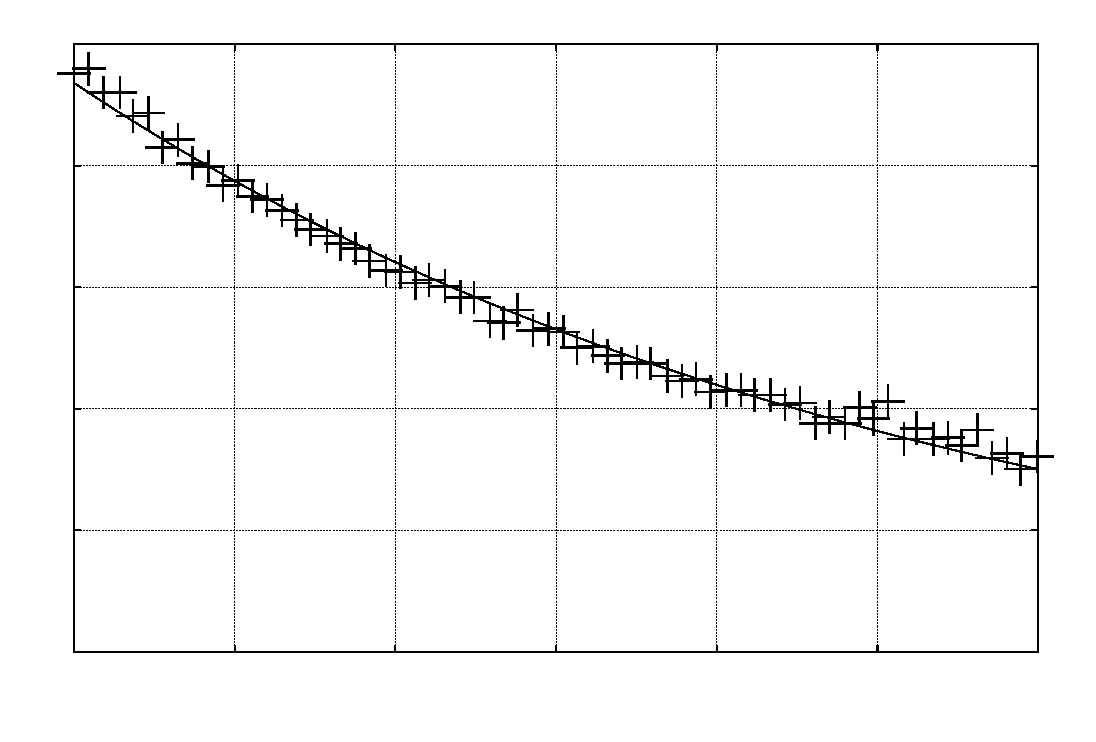
\includegraphics{tlumenymodry}}%
    \gplfronttext
  \end{picture}%
\endgroup

\caption{Časová závislost maximální výchylky při kmitání s modrým tlumícím diskem (hodnoty amplitudy jsou jen poměrné)}
\label{grp::modrytlum}
\end{graph}

Nucené kmity jsme měřili pouze s modrým tlumícím diskem.
Očekávaná resonanční frekvence podle \eqref{eq::resomega} byla \SI{1.096}{\hertz}, nicméně skutečná resonanční frekvence byla přibližně \SI{1.08}{\hertz}.
Naměřené amplitudy $A_v$ a fázové posuny $\gamma$ pro různé frekvence zdroje jsou uvedeny v tabulce \ref{tab::nuceny} a v grafech \ref{grp::nucenyamplitudy} a \ref{grp::nucenyfaze}.
Standardní chybu všech naměřených amplitud a fázových posunutí odhadujeme na \SI{10}{\percent}.


\begin{tabulka}[htbp]
\centering
\begin{tabular}{ccc}
frekvence nutící síly (\si{\hertz}) & amplituda & fázový posun \\ \hline
\num{1.050} & \num{0.19} & \SI{-23}{\degree} \\
\num{1.060} & \num{0.29} & \SI{-28}{\degree} \\
\num{1.070} & \num{0.48} & \SI{-43}{\degree} \\
\num{1.075} & \num{0.77} & \SI{-64}{\degree} \\
\num{1.080} & \num{1.00} & \SI{-101}{\degree} \\
\num{1.085} & \num{0.95} & \SI{-144}{\degree} \\
\num{1.090} & \num{0.80} & \SI{-139}{\degree} \\
\num{1.095} & \num{0.53} & \SI{-182}{\degree} \\
\num{1.100} & \num{0.36} & \SI{-205}{\degree} \\
\num{1.110} & \num{0.25} & \SI{-200}{\degree} \\
\num{1.120} & \num{0.19} & \SI{-203}{\degree} \\
\num{1.130} & \num{0.15} & \SI{-194}{\degree} \\
\end{tabular}
\caption{Nucené kmity s modrým tlumícím diskem ($\delta = \SI{0.038(1)}{\per\second}$)}
\label{tab::nuceny}
\end{tabulka}

\begin{graph}[htbp] 
\centering
% GNUPLOT: LaTeX picture with Postscript
\begingroup
  \makeatletter
  \providecommand\color[2][]{%
    \GenericError{(gnuplot) \space\space\space\@spaces}{%
      Package color not loaded in conjunction with
      terminal option `colourtext'%
    }{See the gnuplot documentation for explanation.%
    }{Either use 'blacktext' in gnuplot or load the package
      color.sty in LaTeX.}%
    \renewcommand\color[2][]{}%
  }%
  \providecommand\includegraphics[2][]{%
    \GenericError{(gnuplot) \space\space\space\@spaces}{%
      Package graphicx or graphics not loaded%
    }{See the gnuplot documentation for explanation.%
    }{The gnuplot epslatex terminal needs graphicx.sty or graphics.sty.}%
    \renewcommand\includegraphics[2][]{}%
  }%
  \providecommand\rotatebox[2]{#2}%
  \@ifundefined{ifGPcolor}{%
    \newif\ifGPcolor
    \GPcolorfalse
  }{}%
  \@ifundefined{ifGPblacktext}{%
    \newif\ifGPblacktext
    \GPblacktexttrue
  }{}%
  % define a \g@addto@macro without @ in the name:
  \let\gplgaddtomacro\g@addto@macro
  % define empty templates for all commands taking text:
  \gdef\gplbacktext{}%
  \gdef\gplfronttext{}%
  \makeatother
  \ifGPblacktext
    % no textcolor at all
    \def\colorrgb#1{}%
    \def\colorgray#1{}%
  \else
    % gray or color?
    \ifGPcolor
      \def\colorrgb#1{\color[rgb]{#1}}%
      \def\colorgray#1{\color[gray]{#1}}%
      \expandafter\def\csname LTw\endcsname{\color{white}}%
      \expandafter\def\csname LTb\endcsname{\color{black}}%
      \expandafter\def\csname LTa\endcsname{\color{black}}%
      \expandafter\def\csname LT0\endcsname{\color[rgb]{1,0,0}}%
      \expandafter\def\csname LT1\endcsname{\color[rgb]{0,1,0}}%
      \expandafter\def\csname LT2\endcsname{\color[rgb]{0,0,1}}%
      \expandafter\def\csname LT3\endcsname{\color[rgb]{1,0,1}}%
      \expandafter\def\csname LT4\endcsname{\color[rgb]{0,1,1}}%
      \expandafter\def\csname LT5\endcsname{\color[rgb]{1,1,0}}%
      \expandafter\def\csname LT6\endcsname{\color[rgb]{0,0,0}}%
      \expandafter\def\csname LT7\endcsname{\color[rgb]{1,0.3,0}}%
      \expandafter\def\csname LT8\endcsname{\color[rgb]{0.5,0.5,0.5}}%
    \else
      % gray
      \def\colorrgb#1{\color{black}}%
      \def\colorgray#1{\color[gray]{#1}}%
      \expandafter\def\csname LTw\endcsname{\color{white}}%
      \expandafter\def\csname LTb\endcsname{\color{black}}%
      \expandafter\def\csname LTa\endcsname{\color{black}}%
      \expandafter\def\csname LT0\endcsname{\color{black}}%
      \expandafter\def\csname LT1\endcsname{\color{black}}%
      \expandafter\def\csname LT2\endcsname{\color{black}}%
      \expandafter\def\csname LT3\endcsname{\color{black}}%
      \expandafter\def\csname LT4\endcsname{\color{black}}%
      \expandafter\def\csname LT5\endcsname{\color{black}}%
      \expandafter\def\csname LT6\endcsname{\color{black}}%
      \expandafter\def\csname LT7\endcsname{\color{black}}%
      \expandafter\def\csname LT8\endcsname{\color{black}}%
    \fi
  \fi
  \setlength{\unitlength}{0.0500bp}%
  \begin{picture}(10204.00,6802.00)%
    \gplgaddtomacro\gplbacktext{%
      \csname LTb\endcsname%
      \put(418,704){\makebox(0,0)[r]{\strut{}}}%
      \csname LTb\endcsname%
      \put(418,1765){\makebox(0,0)[r]{\strut{}}}%
      \csname LTb\endcsname%
      \put(418,2825){\makebox(0,0)[r]{\strut{}}}%
      \csname LTb\endcsname%
      \put(418,3886){\makebox(0,0)[r]{\strut{}}}%
      \csname LTb\endcsname%
      \put(418,4946){\makebox(0,0)[r]{\strut{}}}%
      \csname LTb\endcsname%
      \put(418,6007){\makebox(0,0)[r]{\strut{}}}%
      \csname LTb\endcsname%
      \put(550,484){\makebox(0,0){\strut{} 1.04}}%
      \csname LTb\endcsname%
      \put(1476,484){\makebox(0,0){\strut{} 1.05}}%
      \csname LTb\endcsname%
      \put(2401,484){\makebox(0,0){\strut{} 1.06}}%
      \csname LTb\endcsname%
      \put(3327,484){\makebox(0,0){\strut{} 1.07}}%
      \csname LTb\endcsname%
      \put(4253,484){\makebox(0,0){\strut{} 1.08}}%
      \csname LTb\endcsname%
      \put(5179,484){\makebox(0,0){\strut{} 1.09}}%
      \csname LTb\endcsname%
      \put(6104,484){\makebox(0,0){\strut{} 1.1}}%
      \csname LTb\endcsname%
      \put(7030,484){\makebox(0,0){\strut{} 1.11}}%
      \csname LTb\endcsname%
      \put(7956,484){\makebox(0,0){\strut{} 1.12}}%
      \csname LTb\endcsname%
      \put(8881,484){\makebox(0,0){\strut{} 1.13}}%
      \csname LTb\endcsname%
      \put(9807,484){\makebox(0,0){\strut{} 1.14}}%
      \put(176,3620){\rotatebox{-270}{\makebox(0,0){\strut{}Amplituda}}}%
      \put(5178,154){\makebox(0,0){\strut{}Frekvence budící síly (\si{\hertz})}}%
    }%
    \gplgaddtomacro\gplfronttext{%
    }%
    \gplbacktext
    \put(0,0){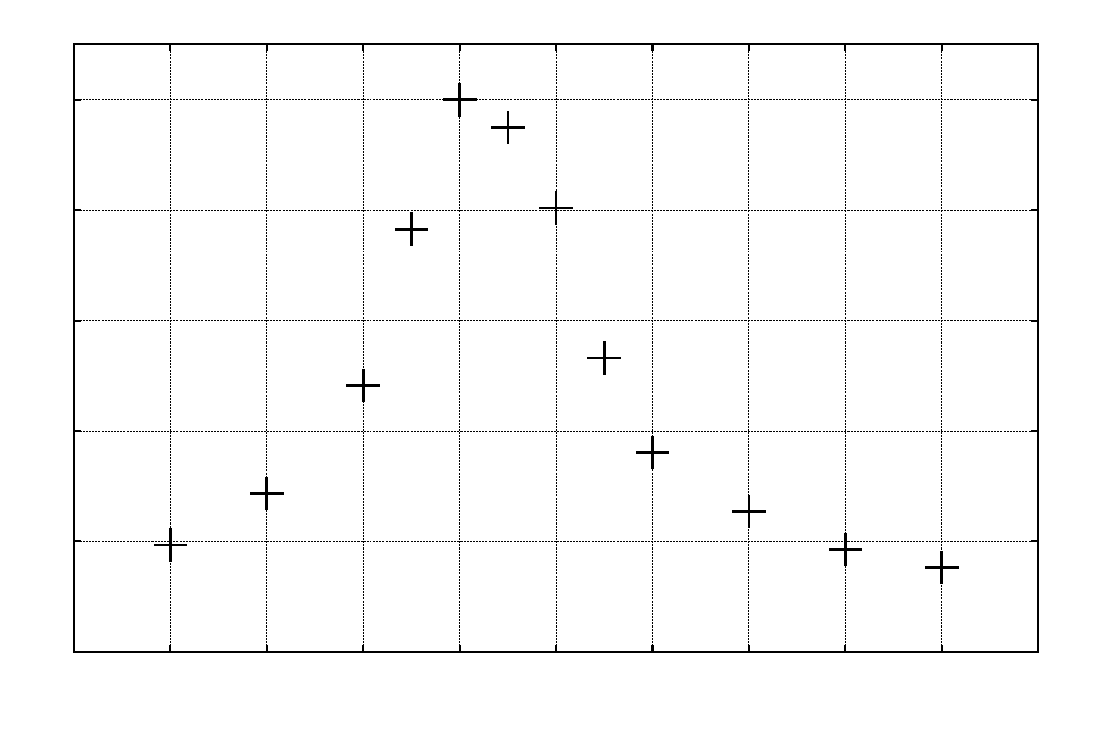
\includegraphics{amp}}%
    \gplfronttext
  \end{picture}%
\endgroup

\caption{Závislost amplitudy na frekvenci budící síly (hodnoty amplitudy jsou jen poměrné)}
\label{grp::nucenyamplitudy}
\end{graph}

\begin{graph}[htbp] 
\centering
% GNUPLOT: LaTeX picture with Postscript
\begingroup
  \makeatletter
  \providecommand\color[2][]{%
    \GenericError{(gnuplot) \space\space\space\@spaces}{%
      Package color not loaded in conjunction with
      terminal option `colourtext'%
    }{See the gnuplot documentation for explanation.%
    }{Either use 'blacktext' in gnuplot or load the package
      color.sty in LaTeX.}%
    \renewcommand\color[2][]{}%
  }%
  \providecommand\includegraphics[2][]{%
    \GenericError{(gnuplot) \space\space\space\@spaces}{%
      Package graphicx or graphics not loaded%
    }{See the gnuplot documentation for explanation.%
    }{The gnuplot epslatex terminal needs graphicx.sty or graphics.sty.}%
    \renewcommand\includegraphics[2][]{}%
  }%
  \providecommand\rotatebox[2]{#2}%
  \@ifundefined{ifGPcolor}{%
    \newif\ifGPcolor
    \GPcolorfalse
  }{}%
  \@ifundefined{ifGPblacktext}{%
    \newif\ifGPblacktext
    \GPblacktexttrue
  }{}%
  % define a \g@addto@macro without @ in the name:
  \let\gplgaddtomacro\g@addto@macro
  % define empty templates for all commands taking text:
  \gdef\gplbacktext{}%
  \gdef\gplfronttext{}%
  \makeatother
  \ifGPblacktext
    % no textcolor at all
    \def\colorrgb#1{}%
    \def\colorgray#1{}%
  \else
    % gray or color?
    \ifGPcolor
      \def\colorrgb#1{\color[rgb]{#1}}%
      \def\colorgray#1{\color[gray]{#1}}%
      \expandafter\def\csname LTw\endcsname{\color{white}}%
      \expandafter\def\csname LTb\endcsname{\color{black}}%
      \expandafter\def\csname LTa\endcsname{\color{black}}%
      \expandafter\def\csname LT0\endcsname{\color[rgb]{1,0,0}}%
      \expandafter\def\csname LT1\endcsname{\color[rgb]{0,1,0}}%
      \expandafter\def\csname LT2\endcsname{\color[rgb]{0,0,1}}%
      \expandafter\def\csname LT3\endcsname{\color[rgb]{1,0,1}}%
      \expandafter\def\csname LT4\endcsname{\color[rgb]{0,1,1}}%
      \expandafter\def\csname LT5\endcsname{\color[rgb]{1,1,0}}%
      \expandafter\def\csname LT6\endcsname{\color[rgb]{0,0,0}}%
      \expandafter\def\csname LT7\endcsname{\color[rgb]{1,0.3,0}}%
      \expandafter\def\csname LT8\endcsname{\color[rgb]{0.5,0.5,0.5}}%
    \else
      % gray
      \def\colorrgb#1{\color{black}}%
      \def\colorgray#1{\color[gray]{#1}}%
      \expandafter\def\csname LTw\endcsname{\color{white}}%
      \expandafter\def\csname LTb\endcsname{\color{black}}%
      \expandafter\def\csname LTa\endcsname{\color{black}}%
      \expandafter\def\csname LT0\endcsname{\color{black}}%
      \expandafter\def\csname LT1\endcsname{\color{black}}%
      \expandafter\def\csname LT2\endcsname{\color{black}}%
      \expandafter\def\csname LT3\endcsname{\color{black}}%
      \expandafter\def\csname LT4\endcsname{\color{black}}%
      \expandafter\def\csname LT5\endcsname{\color{black}}%
      \expandafter\def\csname LT6\endcsname{\color{black}}%
      \expandafter\def\csname LT7\endcsname{\color{black}}%
      \expandafter\def\csname LT8\endcsname{\color{black}}%
    \fi
  \fi
  \setlength{\unitlength}{0.0500bp}%
  \begin{picture}(10204.00,6802.00)%
    \gplgaddtomacro\gplbacktext{%
      \csname LTb\endcsname%
      \put(946,5476){\makebox(0,0)[r]{\strut{}-180}}%
      \csname LTb\endcsname%
      \put(946,4283){\makebox(0,0)[r]{\strut{}-135}}%
      \csname LTb\endcsname%
      \put(946,3090){\makebox(0,0)[r]{\strut{}-90}}%
      \csname LTb\endcsname%
      \put(946,1897){\makebox(0,0)[r]{\strut{}-45}}%
      \csname LTb\endcsname%
      \put(946,704){\makebox(0,0)[r]{\strut{} 0}}%
      \csname LTb\endcsname%
      \put(1078,484){\makebox(0,0){\strut{} 1.04}}%
      \csname LTb\endcsname%
      \put(1951,484){\makebox(0,0){\strut{} 1.05}}%
      \csname LTb\endcsname%
      \put(2824,484){\makebox(0,0){\strut{} 1.06}}%
      \csname LTb\endcsname%
      \put(3697,484){\makebox(0,0){\strut{} 1.07}}%
      \csname LTb\endcsname%
      \put(4570,484){\makebox(0,0){\strut{} 1.08}}%
      \csname LTb\endcsname%
      \put(5443,484){\makebox(0,0){\strut{} 1.09}}%
      \csname LTb\endcsname%
      \put(6315,484){\makebox(0,0){\strut{} 1.1}}%
      \csname LTb\endcsname%
      \put(7188,484){\makebox(0,0){\strut{} 1.11}}%
      \csname LTb\endcsname%
      \put(8061,484){\makebox(0,0){\strut{} 1.12}}%
      \csname LTb\endcsname%
      \put(8934,484){\makebox(0,0){\strut{} 1.13}}%
      \csname LTb\endcsname%
      \put(9807,484){\makebox(0,0){\strut{} 1.14}}%
      \put(176,3620){\rotatebox{-270}{\makebox(0,0){\strut{}Fázový posun (\si{\degree})}}}%
      \put(5442,154){\makebox(0,0){\strut{}Frekvence budící síly (\si{\hertz})}}%
    }%
    \gplgaddtomacro\gplfronttext{%
    }%
    \gplbacktext
    \put(0,0){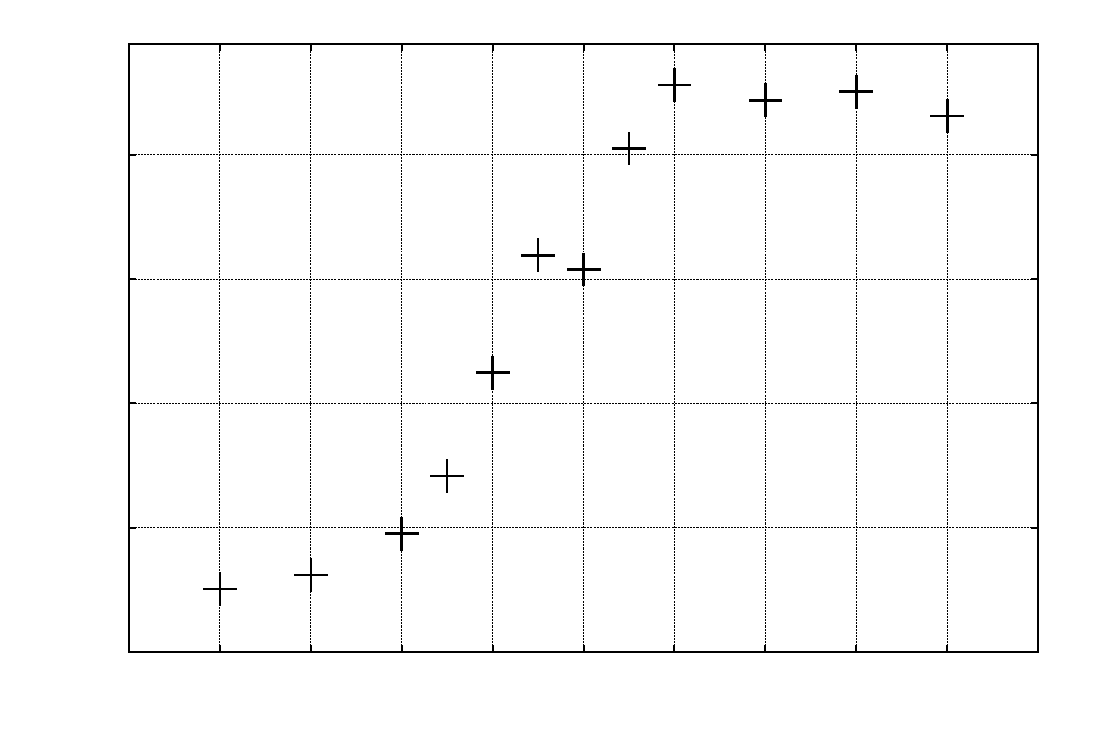
\includegraphics{faz}}%
    \gplfronttext
  \end{picture}%
\endgroup

\caption{Závislost fázového posunu na frekvenci budící síly}
\label{grp::nucenyfaze}
\end{graph}